% =====================================================================
% methods.tex  (upgraded empirical paper)
% Content: the exhaustive, quantitative specification of the model of
% Section~\ref{sec:model}. Pixel geometry and trial timeline of the
% cued change-detection environment(s); the network layer-by-layer
% (conv front-end, recurrent-ViT with element-wise affine feedback,
% spatial xLSTM, distributional actor-critic, JEPA auxiliary); the
% reinforcement-learning objective, replay, target, and curriculum; and
% the three analysis harnesses (attention-clamp / microstimulation, the
% signal-detection read-out, and temporal decoding). THE model is the
% element-wise affine (X' = gamma(H) X + beta(H)) network; it is "the
% model" throughout. No architecture comparison.
% =====================================================================

\section{Methods}
\label{sec:methods}

This section specifies the model, the environments, the training
procedure, and the analysis harnesses in full. Section~\ref{sec:model}
introduced the architecture conceptually and stated the load-bearing
equations; here we give the pixel-level task timeline, the layer-by-layer
network, the exact objective and hyperparameters, and the causal and
read-out analyses that generate the results of
Sections~\ref{sec:detection}--\ref{sec:luomaunsell}. The model is a single
recurrent vision transformer with element-wise affine memory$\to$vision
feedback (Equation~\ref{eq:affine-feedback}), trained end to end with
reinforcement learning and a temporal JEPA auxiliary loss (weight $0.5$). The core causal battery uses one canonical checkpoint;
set-size and paradigm sections use separately trained checkpoints and state that
fact locally. Reported evaluation quantities are single-checkpoint estimates unless
a distribution over trials is stated; they do not estimate between-training-run
uncertainty.

% ---------------------------------------------------------------------
\subsection{The change-detection environment}
\label{sec:methods-env}

The task is a covert cued orientation-change-detection paradigm, rendered
as a short sequence of $50 \times 50$ RGB images with pixel intensities in
$[-1, 1]$, adapted from the cued-attention paradigms of the primate and
psychophysical literature \cite{posner1980_orienting, MullerFindlay1987,
carrasco2011_visual_attention_25y}. The core environment places
$\Nloc = 4$ Gabor stimuli on a $2\times2$ grid, one per $25\times25$
quadrant, indexed row-major so that quadrant, cue, and change indices
coincide (top-left $=$ location $1$, bottom-right $=$ location $4$). Set
size is a manipulated variable (Section~\ref{sec:vda-battery}), but the preserved
comparison is not a pure active-item intervention. The canonical
\texttt{vda1}, \texttt{vda2\_2x2}, and \texttt{vda4} checkpoints all use a
four-token $2\times2$ support with one, two, or four active cells. The
\texttt{vda9} checkpoint uses a $3\times3$ grid, nine active tokens, a
$75\times75$ image, and a correspondingly larger flattened decision readout; its
training support also includes a displayed-validity $p=0$ condition.

The archived checkpoints preserve three historical validity rules. VDA1 is
degenerate because the cue is the only active target. VDA2 was generated by
\texttt{VDASetSizeEnv}, whose invalid branch samples only non-cued active items, so
its displayed and realized validity agree. Archived VDA4 and VDA9 instead use the
legacy sampler, whose invalid branch is uniform over all four or nine locations,
including the cue; their realized cued-change probabilities are respectively
$p+(1-p)/4$ and $p+(1-p)/9$. The separately trained Validity4 checkpoint uses the
same legacy four-location rule as archived VDA4, so target semantics do not confound
that pair. Exact-validity code dated 2026-07-11 applies only to future corrected runs;
no completed corrected derived artifact exists. The
$4\times4$ \texttt{vda16} runs are interrupted pilot runs and are not included
in the quantitative ladder.

\paragraph{Trial timeline.}
A trial is $T = 7$ logical frames indexed $t = 0, \dots, 6$
(Figure~\ref{fig:methods-timeline}):
\begin{itemize}
\item $t = 0$: blank (all-zero) frame.
\item $t = 1$: the \emph{cue}, a coloured disc-and-ring rendered in the
  quadrant of the cued location (a single location drawn uniformly among
  the admissible cue positions); all other quadrants are blank.
\item $t = 2$: blank frame (the delay).
\item $t = 3,4,5,6$: the four oriented Gabor patches, one per location,
  present and held through the end of the trial.
\end{itemize}
The change, when present, occurs at a \emph{fixed} frame, $t = 5$: the
minimum and maximum change frames are both set to $5$, so the model faces
a temporally predictable change onset and the change is visible on frames
$5$ and $6$. On $50\%$ of trials (drawn independently each trial) a change
is present and exactly one patch's orientation steps by $\Delta$ from
$t = 5$ onward; on the remaining $50\%$ no change occurs.

\paragraph{Gabor stimuli and orientation noise.}
Each patch is a Gabor grating (Gaussian envelope $\sigma = 0.5$ on the
$[-1,1]$ patch square, wavelength $\Lambda = 0.3$, aspect ratio $1$, phase
$0$), masked to a central disc, with low-amplitude additive pixel noise
(uniform on $[-0.11, 0.11]$). Each patch is assigned an independent base
orientation drawn uniformly on $[0^\circ, 360^\circ)$ at trial start, and
on \emph{every} stimulus frame an independent orientation jitter is added,
$\eta \sim \sigma_{\mathrm{ori}}\,\mathcal{N}(0,1)$ with
$\sigma_{\mathrm{ori}} = 5^\circ$. The per-frame jitter is the internal
noise the model must integrate through: a single-frame reader cannot
separate a genuine orientation step from the jitter, so detection requires
accumulating evidence across the held stimulus frames. The change is a
sustained orientation offset $\Delta$ added to the changed patch's
orientation from $t = 5$ on (superimposed on the ongoing jitter), with the
signed magnitude drawn per trial as $\Delta \sim \mathcal{U}(-\theta,
\theta)$; $\theta$ is the curriculum-controlled difficulty level
(Section~\ref{sec:methods-curriculum}).

\paragraph{Cue: location, value, and validity.}
The cue at $t = 1$ is a filled central disc (radius $0.32$ of the patch
side) plus a surrounding partial ring (inner/outer radii $0.40$/$0.48$ of
the patch side). Two graded properties are carried on this single cue:
\begin{itemize}
\item \textbf{Validity} is encoded by the \emph{ring completeness}, a
  proportion $p$ drawn uniformly from $\{0.25, 0.5, 0.75, 1.0\}$ (the
  fraction of the ring's circumference that is drawn). For the archived runs,
  VDA2 realizes $p$ exactly, VDA4 and Validity4 realize $p+(1-p)/4$, VDA9
  realizes $p+(1-p)/9$, and VDA1 is degenerate. We report the displayed ring
  proportion and identify the historical rule in cross-checkpoint comparisons.
  The 2026-07-11 exact-validity implementation samples invalid changes only from
  non-cued active locations but has no completed corrected run artifact.
\item \textbf{Value} is encoded by the \emph{cue colour}. In the
  value-directed environment the colour signals the reward for correctly
  detecting a change at the cued location: red $= 5$, green $= 3$,
  blue $= 1$, drawn uniformly per trial. When value is not manipulated the
  cue is white and every correct response earns unit reward.
\end{itemize}

\paragraph{Actions and reward.}
The action space is binary at every frame: \emph{wait} ($0$) or
\emph{declare-change} ($1$). Declaring on or after the change frame on a
genuine reportable-change trial earns the trial's reward magnitude (the
cue-colour value in the value environment, else $1$); declaring before the
change, or on a no-change trial, is a false alarm and ends the trial with
zero reward. Waiting through a no-change trial to the final frame earns the
reward magnitude as a correct rejection. Because both hits \emph{and}
correct rejections are rewarded, an always-wait policy is not trivially
optimal --- it forgoes all hit reward on the $50\%$ of change trials --- and
the model must learn to discriminate a real orientation step from the
per-frame jitter. A trial that is neither declared nor a correct rejection
by the final frame terminates without further reward. This reward
structure corresponds to the value-coupled regime in which correct
responses (both hits and correct rejections) are paid the value magnitude
of the cued location.

\paragraph{Variants.}
The battery of Sections~\ref{sec:value} and~\ref{sec:luomaunsell} realises
established primate paradigms by overriding only the reward, target, or
response rules of the core environment, leaving the timeline, rendering,
and change logic untouched:
\begin{itemize}
\item \textbf{Value-directed (core).} Coloured value cue $+$ validity ring,
  as above; the setting for the core-detection results
  (Section~\ref{sec:detection}).
\item \textbf{Validity (pure spatial cueing).} A separately trained Validity4
  checkpoint with no value colour; a
  white cue whose ring completeness carries validity only, with the cue
  restricted to the two diagonal corners. This checkpoint retains the legacy
  four-location target sampler above, the same historical rule used by archived
  VDA4. It removes the value colour but remains a separately trained rather than
  within-weight VDA4 control
  (Section~\ref{sec:value}).
\item \textbf{Reward-structure sessions (Luo--Maunsell).} Two reward
  regimes on the same stimuli --- a \emph{sensitivity} session in which the
  reward for a correct detection is concentrated at one (cued) location
  (high reward $= 5$ there, $1$ elsewhere), and a \emph{criterion} session
  in which every hit and correct rejection is paid a fixed
  ratio-controlled reward independent of location --- together with a
  response window of $2$ frames after change onset, beyond which an
  undeclared change expires as a miss. This dissociates a sensitivity
  manipulation from a criterion manipulation on matched stimuli
  \cite{luo_maunsell2018_criterion_sensitivity}
  (Section~\ref{sec:luomaunsell}).
\item \textbf{Relative-value (Baruni).} A value-directed session used to
  test whether the model's value sensitivity is relative (context-scaled)
  or absolute (Section~\ref{sec:value}).
\item \textbf{Delay-probe (rehearsal; implemented, not analysed).} The
  implemented environment inserts a transient probe Gabor in the otherwise-blank
  delay frame ($t = 2$) at either the cued (memorised) location or a random
  uncued location, carrying no reward, to test for enhanced processing at the
  memorised location during the delay
  \cite{awh_jonides_reuterlorenz1998_rehearsal}
  (Section~\ref{sec:rehearsal}).
\item \textbf{Attend-here/ignore-here filtering (failed training attempt).}
  Only a change at the cued location is reportable; a foil change should be ignored.
  The attempted checkpoints collapsed to always waiting, so this variant contributes
  no quantitative result. The preserved run-level summary is traced in the Appendix.
\end{itemize}
All environments share the $T = 7$ timeline, the fixed $t = 5$ change, the
$50\%$ change probability, the $\sigma_{\mathrm{ori}} = 5^\circ$ per-frame
jitter, the $\Delta \sim \mathcal{U}(-\theta, \theta)$ change magnitude,
and the curriculum below.

% FIGURE: methods-timeline. Render the 7-frame trial as a filmstrip:
% t0 blank, t1 coloured disc+partial-ring cue in one quadrant, t2 blank,
% t3-6 four Gabors with the changed patch stepping by Delta at t5. Annotate
% the cue's ring completeness (=validity) and colour (=value). Source: a
% single rollout of VDAEnv (envs/base.py rendering); no npz needed.
\begin{figure}[t]
\centering
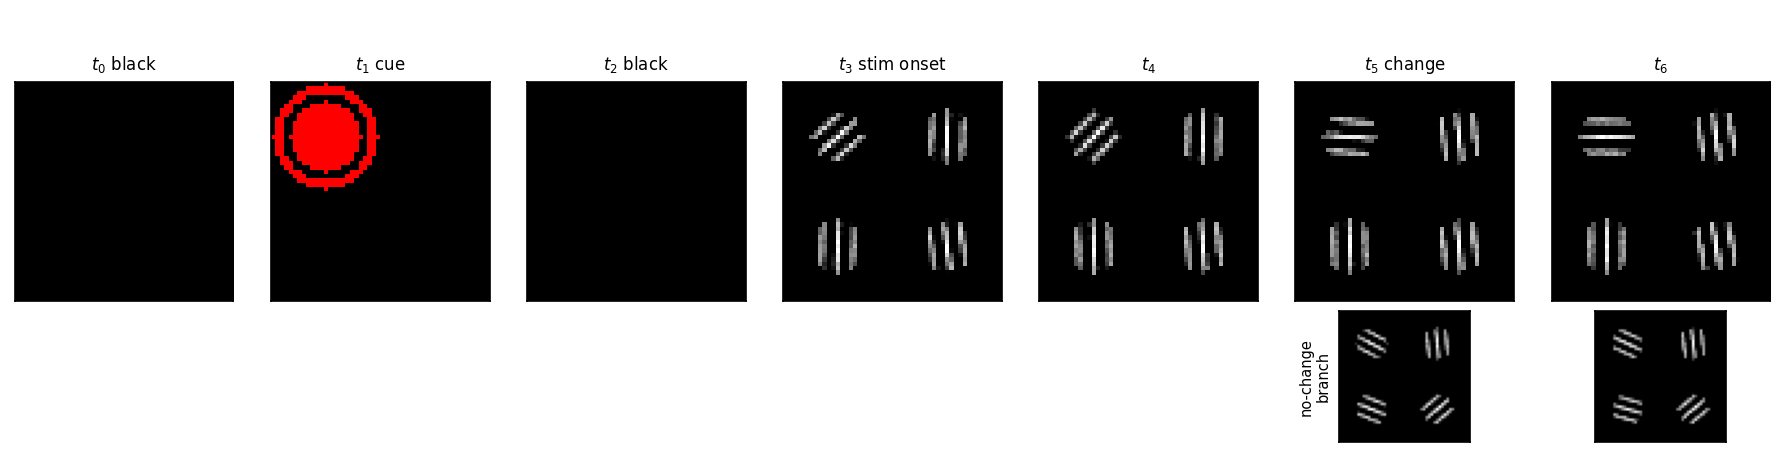
\includegraphics[width=\textwidth]{figures/fig_task_timeline_vda4.png}
\caption{\textbf{Trial timeline of the change-detection environment.} Each
trial is seven frames: a blank, the cue (whose ring completeness signals
validity and whose colour signals value), a blank delay, and four held
Gabor patches, one of which steps in orientation by $\Delta$ at the fixed
change frame $t = 5$ on half of trials. The model chooses \emph{wait} or
\emph{declare-change} at every frame.}
\label{fig:methods-timeline}
\end{figure}

% ---------------------------------------------------------------------
\subsection{Network}
\label{sec:methods-network}

The network chains a convolutional front-end, a recurrent self-attention
encoder with element-wise affine feedback, a per-location spatial working
memory, and a distributional actor--critic, with an auxiliary temporal
self-distillation head; the components were motivated in
Section~\ref{sec:model}. We give the exact layer specification here.

\paragraph{Convolutional front-end.}
In the core four-location checkpoint, each $50\times50$ RGB frame is split into the four $25\times25$ quadrant
patches in row-major order. A single shared squeeze-and-excitation
residual network encodes each patch: a $3\times3$ convolutional stem
($3 \to 32$ channels) followed by three squeeze-and-excitation residual
stages that downsample and grow channels ($32 \to 64$, $25 \to 13$;
$64 \to 128$, $13 \to 7$; $128 \to 128$, $7 \to 7$, added depth without
further downsampling), a global average pool to a $128$-vector, and a
root-mean-square normalisation. Each residual block is
convolution--groupnorm--SiLU $\to$ convolution--groupnorm $\to$
squeeze-and-excitation channel gate $\to$ additive (projected) residual
$\to$ SiLU. Group normalisation (rather than batch normalisation) keeps
the front-end train/eval-identical and stable at the batch size of one
imposed by the online recurrent rollout; root-mean-square normalisation
(rather than a mean-subtracting layer normalisation) preserves the uniform
colour (DC) offset that carries the value cue. The $128$-dimensional patch
embedding $\hat{o}_i$ is concatenated with a one-hot location code
($\Nloc$-dimensional) and a one-hot temporal code ($8$ slots, indexed by
the logical frame), giving a $140$-dimensional token per patch and a token
matrix $X \in \mathbb{R}^{\Nloc \times 140}$ per frame. The front-end
carries $\approx 0.59$~million parameters and is trained end to end from
task reward, with no pretraining and no reconstruction loss.

\paragraph{Recurrent self-attention with element-wise affine feedback.}
The tokens pass through a single recurrent self-attention layer. Before
attending, the tokens are affinely modulated by the previous-step
working-memory state $H \in \mathbb{R}^{\Nloc \times 128}$: a control
vector $b = \tanh(\mathrm{bottleneck}(H))$ of width $64$ is projected to a
per-element scale $\gamma(H)$ and shift $\beta(H)$ of the token shape, and
the tokens are transformed by $X' = \gamma(H) \odot X + \beta(H)$
(Equation~\ref{eq:affine-feedback}). The scale bias is initialised to one
and the shift to zero, so $X' = X$ at initialisation and the layer begins
as ordinary self-attention; the memory's gain-and-bias field is learned.
The modulated tokens undergo standard scaled dot-product self-attention
over the $\Nloc$ locations, $Q = X'W_Q$, $K = X'W_K$, $V = X'W_V$,
$A = \mathrm{softmax}(QK^{\top}/\sqrt{d})$, $Z = X + AV$
(Equation~\ref{eq:self-attention}), with the raw tokens $X$ retained as a
residual so the current frame always reaches memory regardless of the
attention weights. The attention matrix $A \in \mathbb{R}^{\Nloc \times
\Nloc}$ is the model's internal allocation of processing across space; its
row-marginal $\alpha_i$ is the attention share on location $i$, and is the
quantity read out and manipulated in the analyses below. The pre-softmax
attention logits accept an additive per-key clamp used only in analysis
(Section~\ref{sec:methods-clamp}); it is inert during training.

\paragraph{Spatial working memory.}
The contextualised tokens $Z$ are integrated across the trial by an
extended-LSTM (xLSTM) cell applied per location with shared parameters but
a private state per patch, producing a $128$-dimensional memory vector
$H_i$ per location. Writing the stabilised update, the input, forget,
output, and cell-input pre-activations are $\tilde{I} = ZW_i + HR_i$,
$\tilde{F} = ZW_f + HR_f$, $\tilde{O} = ZW_o + HR_o$, $\tilde{U} = ZW_u +
HR_z$ (input maps $W \in \mathbb{R}^{140\times128}$ biased, recurrent maps
$R \in \mathbb{R}^{128\times128}$ bias-free); the log-domain stabiliser is
$M = \max(\tilde{F} + M_{\mathrm{prev}}, \tilde{I})$ with
$I = \exp(\tilde{I} - M)$ and $F = \exp(\tilde{F} + M_{\mathrm{prev}} -
M)$; and the state updates are $O = \sigma(\tilde{O})$, $U =
\tanh(\tilde{U})$, $N = F \odot N_{\mathrm{prev}} + I$, $C =
C_{\mathrm{prev}} \odot F + U \odot I$, $H = O \odot (C / N)$, with the
state $(H, C, N, M)$ per patch initialised to zero. The stabilised
exponential gates give a controllable retention time-constant, so the
memory can encode cue information across the blank
delay and accumulate weak orientation evidence across the stimulus
frames. The memory state at frame $t$ is the $H$ that drives the affine
feedback (Equation~\ref{eq:affine-feedback}) at frame $t+1$, closing the
perception--memory loop.

\paragraph{Distributional actor--critic.}
The $\Nloc$ per-location memory vectors are flattened into a single
$\Nloc \times 128$-dimensional readout ($512$ dimensions in the core
four-token checkpoint and $1152$ in \texttt{vda9}); the spatial structure is
discarded at the decision stage. Two heads that share no parameters read
it, each a three-layer feed-forward trunk (width $256$, ELU
nonlinearities). The \emph{actor} maps the readout to logits over the two
actions and is biased at initialisation toward \emph{wait}
(bias $[0.0, -1.5]$) so the model does not begin by declaring on every
frame. The \emph{critic} is a distributional quantile head: it outputs
$5$ return quantiles per action (quantile-regression value head), and the
state value is recovered as the action-probability-weighted mean of the
per-action quantile means. The decision is made online, frame by frame,
which gives the model a reaction time and hence a chronometric function.

\paragraph{Auxiliary temporal self-distillation.}
A joint-embedding predictive self-distillation head (a temporal V-JEPA
objective with DINO-style centering) reads the memory cell at each
location and predicts, for the same location one frame ahead, the soft
prototype assignment of an exponential-moving-average teacher copy of the
network. The head emits, per location, $4$ independent softmax
distributions over $256$ prototypes each. It has no direct forward connection to the actor, critic, attention logits,
or next recurrent state. Its loss nevertheless backpropagates through shared
representations and can therefore influence the learned features and behaviour.

The core model uses a per-location memory width of $d_{\mathrm{mem}} = 128$
throughout; the working-memory-capacity manipulation of
Section~\ref{sec:capacity} varies $d_{\mathrm{mem}}$ (128 versus 256) with
all else fixed.

% ---------------------------------------------------------------------
\subsection{Reinforcement-learning objective}
\label{sec:methods-training}

The total training objective combines an off-policy maximum-a-posteriori
actor--critic objective from sparse task reward with the temporal JEPA
self-distillation loss (weight $0.5$). The reinforcement component uses a
distributional critic, prioritised episodic replay, and an exponential-moving-average target.

\paragraph{Actor.}
The actor is updated by a maximum-a-posteriori policy-optimisation step:
an expectation step reweights actions by their advantage under the
exponential-moving-average reference policy at temperature $\eta = 0.1$,
followed by a weighted maximisation with a behavioural-cloning term
(behavioural-cloning weight $0.1$; $0$ recovers pure policy optimisation,
$1$ pure cloning) and an entropy regulariser (coefficient $0.01$). The
reference policy in the expectation step is the target network, not the
online network.

\paragraph{Critic.}
The critic is trained by a quantile-regression temporal-difference loss
over its $5$ return quantiles, with quantile-Huber threshold
$\kappa = 1.0$ and value-loss weight $0.5$. The bootstrap target is
computed from the exponential-moving-average target network. The discount
is $\gamma = 0.95$.

\paragraph{Replay and target.}
Learning uses prioritised \emph{episodic} replay: complete trials are
stored in a first-in-first-out buffer (capacity $1000$ episodes) and
sampled by priority (priority exponent $0.6$, importance-sampling exponent
annealed $0.4 \to 1.0$, priority clip $50$), with $4$ replayed episodes
alongside the fresh on-policy episodes each iteration, so informative
whole trials are revisited in proportion to their surprise. The target
network is an exponential moving average of the online network (decay
$0.995$, applied to parameters and buffers each iteration), and supplies
both the critic bootstrap target and the actor's reference policy,
replacing a hard periodic copy.

\paragraph{JEPA teacher.}
The self-distillation teacher is a separate exponential-moving-average copy
of the network (parameters only, decay $0.996$, decoupled from the
reinforcement-learning target), and the student at frame $t$ predicts the
teacher's soft assignment at frame $t+1$. DINO-style centering uses
centre-momentum $0.9$; the student temperature is $0.1$ and the teacher
temperature is warmed from $0.04$ to $0.07$ over the first $300$
iterations. The self-distillation loss enters the total objective with
weight $0.5$.

\paragraph{Optimisation.}
Parameters are optimised with a learning rate of $3\times10^{-4}$ and
gradient-norm clipping at $0.5$. Each iteration collects $8$ episodes, with a
burn-in of $20$ iterations before replay-based updates begin. Each canonical
affine $d_{\mathrm{mem}}=128$ VDA1/VDA2\_2x2/VDA4/VDA9 run has one preserved metrics file with
20{,}000 rows ending at logged iteration 19{,}999 and one canonical final
checkpoint. This documents a completed logged phase, not formal convergence.
Resume jobs can reset iteration counters and overwrite \texttt{metrics.csv}, so
cumulative lifetime updates cannot be reconstructed from those files.

\paragraph{Difficulty curriculum.}
\label{sec:methods-curriculum}
Difficulty is set by the change-magnitude bound $\theta$ in
$\Delta \sim \mathcal{U}(-\theta, \theta)$, and is shrunk by a performance
curriculum so the model is always trained near the edge of its competence.
$\theta$ starts at $65^\circ$; correctness is averaged over
\emph{non-overlapping} windows of $1000$ trials, and whenever a completed
window is solved at $\geq 85\%$ correct, $\theta$ is reduced by $3^\circ$,
floored at $8^\circ$. Shrinking $\theta$ makes changes smaller and thus
harder to discriminate against the fixed $5^\circ$ per-frame jitter, so the
model is driven toward finer sensitivity as it improves. Because the
change is signed and drawn symmetrically, at any $\theta$ the trial pool
spans the full range of change magnitudes up to $\theta$, and psychometric
functions are constructed by binning trials on the realised $|\Delta|$
rather than on $\theta$.

% ---------------------------------------------------------------------
\subsection{Analysis harnesses}
\label{sec:methods-analysis}

Each analysis is run off-policy on the frozen checkpoint named by its result
section, by re-encoding whole trial sequences and reading out (or intervening on)
the internal quantities. Unless stated, an analysis condition is estimated
over a fixed batch of freshly sampled trials at the model's
curriculum-hardened operating point, and the change magnitude is set to a
diagnostic value (e.g.\ $\Delta = 18^\circ$ or $\Delta = 28^\circ$) or
swept to build a psychometric function.

% .....................................................................
\subsubsection{Attention clamp: microstimulation and graded biasing}
\label{sec:methods-clamp}

The single causal lever is an additive bias on the pre-softmax attention
logits of a chosen key location, applied at inference only. Writing a bias
$\beta_j$ on the logits of key location $j$ shifts the softmax allocation
$A$ toward ($\beta_j > 0$) or away from ($\beta_j < 0$) that location,
without altering the trained weights. Figures parameterise the intervention by a
nominal clamp value, denoted $\alpha_{\mathrm{nom}}$, which is mapped to this
additive logit bias. It is an intervention setting, not a measured post-softmax
attention share; realized attention is read separately from $A$. We use the lever in three modes, all
mirroring interventional primate paradigms in which a spatial priority
signal is injected or removed:
\begin{itemize}
\item \textbf{Graded biasing.} Sweeping the nominal clamp from suppress to
  enhance, mapping it to a negative or positive $\beta$ on the cued key, and
  reading out signal-detection quantities and behaviour against that nominal
  setting (Section~\ref{sec:methods-sdt},
  Section~\ref{sec:det-sdt}). This is a within-model dose--response on the
  attentional allocation.
\item \textbf{Hard override.} Clamping the allocation onto a specified
  location ($\alpha \to 1$ there) on trials whose change is elsewhere, to
  test whether forcing attention onto (or off) a location changes
  detection --- the analogue of enhancing or inactivating a spatial
  priority representation \cite{MullerFindlay1987}.
\item \textbf{Microstimulation.} Injecting attention (positive bias) onto a
  location on \emph{no-change} trials, to test whether surplus priority
  conjures a false detection, and whether the evoked percept is spatially
  gated to the monitored location (Section~\ref{sec:det-microstim}). The
  injection strength is swept and the induced false-alarm rate recorded at
  the cued versus an uncued site, the causal converse of the criterion
  read-out.
\end{itemize}

% .....................................................................
\subsubsection{Signal-detection read-out}
\label{sec:methods-sdt}

Behaviour is scored in signal-detection terms on matched change and
no-change trials. A \emph{hit} is a declare-change response on or after the
change on a genuine change trial; a \emph{false alarm} is a declare
response on a no-change trial; the hit rate $H$ and false-alarm rate
$F$ over a trial batch yield sensitivity $d' = \Phi^{-1}(H) -
\Phi^{-1}(F)$ and criterion $c = -\tfrac12[\Phi^{-1}(H) + \Phi^{-1}(F)]$,
with $\Phi^{-1}$ the standard-normal quantile function and rates clipped
away from $0$ and $1$ before inversion. The central signal-detection
analysis pairs this read-out with the graded attention clamp
(Section~\ref{sec:methods-clamp}): $d'$ and $c$ are computed as a function
of the nominal clamp setting (with realized attention reported separately), isolating how attention
moves sensitivity versus decision criterion
(Section~\ref{sec:det-sdt}). In the Luo--Maunsell reward-structure
sessions (Section~\ref{sec:luomaunsell}) the same $d'$/$c$ read-out is
computed across the sensitivity and criterion sessions to test the
sensitivity$\to d'$, criterion$\to c$ double dissociation
\cite{luo_maunsell2018_criterion_sensitivity}. Policy entropy (of the
actor's action distribution) and critic quantile spread are read out
alongside $d'$ and $c$ under the clamp to quantify decision confidence and
value uncertainty (Section~\ref{sec:det-uncertainty}).

% .....................................................................
\subsubsection{Temporal decoding from working memory}
\label{sec:methods-decoding}

To ask what the memory holds and when, a linear decoder is trained to read
each trial-defining variable from the flattened working-memory state at
each frame. On a batch of trials, cross-validated balanced accuracy is
reported per frame $t = 1, \dots, 6$ for four variables: cue value (cue
colour), cue validity (displayed ring proportion), change presence, and
change location. Balanced accuracy is referenced against the chance level
of each variable's label set. This yields a per-variable time course
across the trial --- for example, whether a variable is latched at the cue
and maintained, perceived transiently and then discarded, or constructed
online at the change frame --- and is the read-out behind the memory-code
analysis of Section~\ref{sec:det-decoding}. The same decoder, applied to
the value-directed versus pure-validity environments, estimates whether a
variable remains linearly recoverable at the sampled frames. Manuscript claims
about change location are restricted to the supported VDA4 analysis: the
2026-07-07 legacy \texttt{decode.npz} VDA2 and VDA9 change-location fields were
generated with degenerate labels and are not interpreted here. Other fields in
that archive, including the validity time courses reported in
Section~\ref{sec:vda-decode}, are separate decoder targets and remain usable.
No cue-location decoder was fitted across the blank delay; later cue-directed
attention is reported as re-acquisition compatible with maintenance, not as a
decoded maintained cue-location representation.

For VDA4 validity, the canonical manuscript series is the validity field for the
affine-feedback VDA4 condition in the preserved \texttt{decode.npz} archive. It
was generated by the set-size decoder harness on the canonical 128-memory VDA4
checkpoint; the evidence ledger records the full artifact paths. The series is
$0.773$ at $t=1$, $0.296$ at $t=2$, and near four-way chance thereafter
(mean $t=2$--$6$: $0.309$). A distinct exploratory deep-dive archive used a
different sampling harness but does not independently encode sufficient checkpoint
provenance for its validity series, so it is not used in the manuscript. The
versioned corrected decoder collector writes beneath the dated derived-output
directory; a completed corrected artifact remains pending, while the preserved
legacy validity fields remain usable.

% ---------------------------------------------------------------------
\subsection{Reproducibility and implementation}
\label{sec:methods-repro}

Each reported analysis identifies a frozen set of weights, and reported condition
means are estimated over freshly sampled trial batches at the operating point stated
with each result. The set-size summaries use one canonical affine-feedback checkpoint per condition;
the current figures do not provide between-seed uncertainty or saved trial-level
confidence intervals. The manuscript does not use the legacy high-token
\texttt{crossattn1} clamp outputs, whose location indexing failed to bias both the
image and corresponding memory key at VDA9; all reported set-size clamp curves are
for affine feedback. The environments, network,
training loop, and analysis harnesses are implemented in Python with
PyTorch. Training and analysis were run on Apple-silicon (MPS) and CPU
backends; results are backend-independent, and the analyses that generate
the reported numbers are run on the frozen trained network.
